\chapter{Resultados Obtenidos y Análisis}
\textcolor{red}{Falta redactar, pero están todos los resultados. Revisar captions de figuras}
\section{Caso I: Høvsøre s/DA}
\newpage
\begin{figure}[H]
	\centering
	\begin{minipage}{0.5\linewidth}
		\center\hspace{0.3cm}(a)
	\end{minipage}%
	\begin{minipage}{0.5\linewidth}
		\center\hspace{0.3cm}(b)
	\end{minipage}%
	
	\includegraphics[width=0.5\linewidth,page=10,trim={2.5cm 6.2cm 1cm 4.5cm},clip]{Imagenes/06/hov/eta1_u}%
	\includegraphics[width=0.5\linewidth,page=10,trim={2.5cm 6.2cm 1cm 4.5cm},clip]{Imagenes/06/hov/eta1_v}%
	
	\center{\hspace{0.3cm}(c)}
	
	\includegraphics[width=0.5\linewidth,page=10,trim={2.5cm 6.2cm 1cm 4.5cm},clip]{Imagenes/06/hov/eta1_V}%
	\caption{(a) Componente $u$ de la velocidad en el primer nivel de la coordenada vertical ($z_1=5.25$ [m]) para las 15:00. (b) Idéntico al anterior pero para la componente $v$. (c) Magnitud del campo de velocidad.}
	\label{fig:06_hov_eta1}
\end{figure}

\begin{figure}[H]
	\centering
	\includegraphics[width=1\linewidth,trim={9mm 63mm 10mm 55mm},clip]{Imagenes/06/hov/ts_v}%
	
	\includegraphics[width=1\linewidth,trim={12mm 55mm 10mm 55mm},clip]{Imagenes/06/hov/ts_o}%
	\caption{Serie de tiempo para la rapidez instantánea del viento $V$ y su dirección en la ubicación del mástil meteorológico. La línea continua corresponde a lo datos simulados interpolados a las alturas de medición (solo para $V$) y la línea punteada a los datos medidos en el mástil.}
	\label{fig:06_hov_ts}
\end{figure}

\begin{figure}[H]
	\begin{minipage}{0.5\linewidth}
		\centering{\hspace{0.9cm}(a)}
	\end{minipage}%
	\begin{minipage}{0.5\linewidth}
		\centering{\hspace{0.6cm}(b)}
	\end{minipage}%
	
	\begin{minipage}{0.5\linewidth}
		\centering
		\includegraphics[width=0.9\linewidth,trim={0cm 5mm 0cm 0mm},clip]{Imagenes/06/hov/pbl}%
	\end{minipage}%
	\begin{minipage}{0.5\linewidth}
		\centering
		\includegraphics[width=0.9\linewidth,trim={0cm 5mm 0cm 0cm},clip]{Imagenes/06/hov/temp_profile}%
	\end{minipage}%
	
	\caption{Ciclo diurno-nocturno del perfil de temperatura potencial en el mástil meteorológico. (a) Resultados cada 20 minutos del perfil de $\theta$. (b) Corresponde al detalle del perfil dentro de la capa límite atmosférica ($\delta \approx 750$ [m]).}
	\label{fig:06_hov_pbl}
\end{figure}

\begin{figure}[H]
	\begin{minipage}{0.33\linewidth}
		\centering \hspace{1.5cm}(a)
	\end{minipage}%
	\begin{minipage}{0.33\linewidth}
		\centering \hspace{1cm}(b)
	\end{minipage}%
	\begin{minipage}{0.33\linewidth}
		\centering \hspace{1cm}(c)
	\end{minipage}%
	\vspace{-3mm}
	\begin{center}
	\includegraphics[height=0.62\linewidth,page=37,trim={35mm 10mm 41mm 25mm},clip]{Imagenes/06/hov/9u}%
	\includegraphics[height=0.62\linewidth,page=37,trim={48mm 10mm 41mm 25mm},clip]{Imagenes/06/hov/9v}%
	\includegraphics[height=0.62\linewidth,page=37,trim={48mm 10mm 41mm 25mm},clip]{Imagenes/06/hov/9V}%
	\end{center}
	\caption{Comparación de la simulación (línea continua) con la simulación de Peña et. al. en el 2013 (línea punteada) y valores medidos para (a) componente $u$ de la velocidad del viento, (b) componente $v$ y (c) magnitud de la velocidad del viento. Los datos corresponden a promedios temporales entre las 12:00 y 14:00, y han sido rotados de tal forma que su dirección sea 0$^\circ$ a los 10m.}
	\label{fig:06_hov_peña}
\end{figure}

\begin{figure}[H]
	\begin{minipage}{0.33\linewidth}
		\centering \hspace{1cm}(a)
	\end{minipage}%
	\begin{minipage}{0.33\linewidth}
		\centering \hspace{0.8cm}(b)
	\end{minipage}%
	\begin{minipage}{0.33\linewidth}
		\centering \hspace{0.5cm}(c)
	\end{minipage}%
	\vspace{-4mm}
	\begin{center}
	\includegraphics[height=0.5\linewidth,page=1,trim={6mm 5mm 3mm 0mm},clip]{Imagenes/06/hov/mean_data}%
	\includegraphics[height=0.5\linewidth,page=2,trim={12mm 5mm 3mm 0mm},clip]{Imagenes/06/hov/mean_data}%
	\includegraphics[height=0.5\linewidth,page=3,trim={12mm 5mm 3mm 0mm},clip]{Imagenes/06/hov/mean_data}%
	\end{center}
	\caption{Variables adimensionalizadas ($u_* = 0.552$ [m/s]) de segundo orden para el caso de Høvsøre promediados entre las 12:00 y las 15:00 (atmósfera neutra, terreno plano homogéneo). (a) Energía cinética turbulenta de submalla, (b) Gradiente de velocidad, (c) Esfuerzo turbulento. }
	\label{fig:06_hov_mean_secondorder}
\end{figure}

\begin{figure}[H]
	\centering
	\includegraphics[width=1.0\linewidth,page=1,trim={3mm 5mm 3mm 3mm},clip]{Imagenes/06/hov/spectra}%
	\caption{Espectros de energía para la componente horizontal del viento a distintos niveles verticales en el dominio d07 caso Høvsøre.}
	\label{fig:06_hov_spectrum}
\end{figure}

\section{Caso I: Høvsøre c/DA}

\begin{figure}[H]
	\centering
	\includegraphics[width=1\linewidth,trim={9mm 63mm 10mm 55mm},clip]{Imagenes/06/hov_da/ts_v}%
	
	\includegraphics[width=1\linewidth,trim={12mm 55mm 10mm 55mm},clip]{Imagenes/06/hov_da/ts_o}%
	\caption{Serie de tiempo para la rapidez instantánea del viento $V$ y su dirección en la ubicación del mástil meteorológico para el caso con asimilación de datos. La línea continua corresponde a lo datos simulados interpolados a las alturas de medición (solo para $V$) y la línea punteada a los datos medidos en el mástil.}
	\label{fig:06_hov_da_ts}
\end{figure}



\begin{figure}[H]
	\begin{minipage}{0.33\linewidth}
		\centering \hspace{1cm}(a)
	\end{minipage}%
	\begin{minipage}{0.33\linewidth}
		\centering \hspace{0.8cm}(b)
	\end{minipage}%
	\begin{minipage}{0.33\linewidth}
		\centering \hspace{1cm}(c)
	\end{minipage}%
	\vspace{-3mm}
	\begin{center}
	\includegraphics[height=0.61\linewidth,page=37,trim={35mm 10mm 38mm 25mm},clip]{Imagenes/06/hov_da/9u}%
	\includegraphics[height=0.61\linewidth,page=37,trim={48mm 10mm 38mm 25mm},clip]{Imagenes/06/hov_da/9v}%
	\includegraphics[height=0.61\linewidth,page=37,trim={48mm 10mm 38mm 25mm},clip]{Imagenes/06/hov_da/9V}%
	\end{center}
	\caption{Comparación de la simulación con DA (línea continua) con la simulación de Peña et. al. en el 2013 (linea punteada) y valores medidos para (a) componente $u$ de la velocidad del viento, (b) componente $v$ y (c) magnitud de la velocidad del viento. Los datos corresponden a promedios temporales entre las 12:00 y 14:00, y han sido rotados de tal forma que su dirección sea 0$^\circ$ a los 10m.}
	\label{fig:06_hov_da_peña}
\end{figure}

\begin{figure}[H]
	\begin{minipage}{0.33\linewidth}
		\centering \hspace{1cm}(a)
	\end{minipage}%
	\begin{minipage}{0.33\linewidth}
		\centering \hspace{0.8cm}(b)
	\end{minipage}%
	\begin{minipage}{0.33\linewidth}
		\centering \hspace{0.5cm}(c)
	\end{minipage}%
	\vspace{-4mm}
	\begin{center}
		\includegraphics[height=0.5\linewidth,page=1,trim={6mm 5mm 3mm 0mm},clip]{Imagenes/06/hov_da/mean_data}%
		\includegraphics[height=0.5\linewidth,page=2,trim={12mm 5mm 3mm 0mm},clip]{Imagenes/06/hov_da/mean_data}%
		\includegraphics[height=0.5\linewidth,page=3,trim={12mm 5mm 3mm 0mm},clip]{Imagenes/06/hov_da/mean_data}%
	\end{center}
	\caption{Variables adimensionalizadas ($u_* = 0.527$ [m/s]) de segundo orden para el caso de Høvsøre con DA promediados entre las 12:00 y las 15:00 (atmósfera neutra, terreno plano homogéneo). (a) Energía cinética turbulenta de submalla, (b) Gradiente de velocidad, (c) Esfuerzo turbulento. }
	\label{fig:06_hov_da_mean_secondorder}
\end{figure}

\begin{figure}[H]
	\centering
	\includegraphics[width=1.0\linewidth,page=1,trim={3mm 5mm 3mm 3mm},clip]{Imagenes/06/hov_da/spectra}%
	\caption{Espectros de energía para la componente horizontal del viento a distintos niveles verticales en el dominio d07 caso Høvsøre con DA.}
	\label{fig:06_hov_da_spectrum}
\end{figure}

\begin{table}[h!]
	\caption{Comparación de métricas para el caso I Høvsøre.}
	\label{tab:06_hov_mae_rmse}
	\centering%\footnotesize
	\begin{tabular}{lcc}
		\toprule
		& Sin DA & Con DA \\
		\midrule
		MAE & 2.41091 m/s & 2.16742 m/s \\
		RMSE & 2.80142 m/s& 2.55778 m/s\\
		\bottomrule
	\end{tabular}
\end{table}

















\newpage
\section{Caso II: Bolund s/DA}

\begin{figure}[H]
	\begin{minipage}{0.5\linewidth}
		\centering{\hspace{0.9cm}(a)}
	\end{minipage}%
	\begin{minipage}{0.5\linewidth}
		\centering{\hspace{0.6cm}(b)}
	\end{minipage}%
	
	\begin{minipage}{0.5\linewidth}
		\centering
		\includegraphics[width=0.9\linewidth,trim={0cm 5mm 0cm 0mm},clip]{Imagenes/06/bol/mean_pbl}%
	\end{minipage}%
	\begin{minipage}{0.5\linewidth}
		\centering
		\includegraphics[width=0.9\linewidth,trim={0cm 5mm 0cm 0cm},clip]{Imagenes/06/bol/mean_profile}%
	\end{minipage}%
	
	
	
	\caption{Ciclo horario del perfil de temperatura potencial promedio de los 8 mástiles. (a) Resultados cada 10 minutos del perfil de $\theta$. (b) Corresponde al detalle del perfil dentro de la capa límite atmosférica con resultados cada 15 minutos ($\delta\approx300$ [m]).}
	\label{fig:06_bol_pbl}
\end{figure}

\begin{figure}[H]
	\begin{minipage}{0.5\linewidth}
		\centering
		\hspace{1cm}(a)
	\end{minipage}%
	\begin{minipage}{0.5\linewidth}
		\centering
		\hspace{-1cm}(b)
	\end{minipage}%
	
	\begin{minipage}{0.5\linewidth}
		\centering
		\includegraphics[height=0.70\linewidth,page=73,trim={12mm 31mm 50mm 20mm},clip]{Imagenes/06/bol/eta1}%
	\end{minipage}%
	\begin{minipage}{0.5\linewidth}
		\centering
		\includegraphics[height=0.70\linewidth,page=85,trim={37mm 31mm 20mm 20mm},clip]{Imagenes/06/bol/eta1}%
	\end{minipage}%
	\vspace{1mm}
	
	\begin{minipage}{0.5\linewidth}
		\centering
		\hspace{1cm}(c)
	\end{minipage}%
	\begin{minipage}{0.5\linewidth}
		\centering
		\hspace{-1cm}(d)
	\end{minipage}%
	
	\begin{minipage}{0.5\linewidth}
		\centering
		\includegraphics[height=0.73\linewidth,page=97,trim={12mm 23mm 50mm 20mm},clip]{Imagenes/06/bol/eta1}%
	\end{minipage}%
	\begin{minipage}{0.5\linewidth}
		\centering
		\includegraphics[height=0.73\linewidth,page=109,trim={37mm 23mm 20mm 20mm},clip]{Imagenes/06/bol/eta1}%
	\end{minipage}%
	\caption{Lineas de flujo para la solución numérica en Bolund en el primer nivel ($z_1 = 1.12$ [m]) en las horas (a) 12:00, (b) 13:00, (c) 14:00, (d) 15:00.}
	\label{fig:06_bol_st}
\end{figure}

\begin{figure}[H]
	\centering
	\includegraphics[width=0.90\linewidth,trim={0mm 202.0mm 111mm 106mm},clip]{Imagenes/06/bol/1200rot}\\%
	\includegraphics[width=0.90\linewidth,trim={0mm 202.0mm 111mm 106mm},clip]{Imagenes/06/bol/1300rot}\\%
	\includegraphics[width=0.90\linewidth,trim={0mm 202.0mm 111mm 106mm},clip]{Imagenes/06/bol/1400rot}\\%
	\includegraphics[width=0.90\linewidth,trim={0mm 180.0mm 111mm 106mm},clip]{Imagenes/06/bol/1500rot}%
	\caption{Contornos de rapidez del viento para la sección de corte a 240$^\circ$ en Bolund. Se muestran los resultados para las 12:00, 13:00, 14:00 y 15:00 horas.}
	\label{fig:06_bol_cross}
\end{figure}

\begin{figure}[H]
	\begin{minipage}{0.5\linewidth}
		\centering{\hspace{0.9cm}(a)}
	\end{minipage}%
	\begin{minipage}{0.5\linewidth}
		\centering{\hspace{0.6cm}(b)}
	\end{minipage}%
	
	\begin{minipage}{0.5\linewidth}
		\centering
		\includegraphics[width=0.7\linewidth,trim={4.5cm 12mm 4.3cm 20mm},clip]{Imagenes/06/bol/V_referencia}%
	\end{minipage}%
	\begin{minipage}{0.5\linewidth}
		\centering
		\includegraphics[width=0.7\linewidth,trim={4.5cm 12mm 4.3cm 20mm},clip]{Imagenes/06/bol/tke_referencia}%
	\end{minipage}%
	
	
	
	\caption{Perfiles promedio referenciales en el flujo no perturbado para: (a) Rapidez del viento (en línea punteada se presenta la condición de contorno presentada por Bechmann et. al., 2011) (b) Intensidad de energía cinética turbulenta (sgs).}
	\label{fig:06_bol_referencia}
\end{figure}

\begin{figure}[H]
	\centering
	\includegraphics[width=0.95\linewidth,trim={12mm 84mm 10mm 74mm},page=1,clip]{Imagenes/06/bol/speedup}\\%
	\includegraphics[width=0.95\linewidth,trim={12mm 84mm 10mm 74mm},page=13,clip]{Imagenes/06/bol/speedup}\\%
	\includegraphics[width=0.95\linewidth,trim={12mm 84mm 10mm 74mm},page=25,clip]{Imagenes/06/bol/speedup}\\%
	\includegraphics[width=0.95\linewidth,trim={12mm 84mm 10mm 74mm},page=37,clip]{Imagenes/06/bol/speedup}\\%
	\includegraphics[width=0.95\linewidth,trim={-11mm 193mm 115mm 112mm},clip]{Imagenes/06/bol/cross_height}\\%
	\caption{Speedup en los primeros 3 niveles del modelo ($1.1$ [m] azul; $3.4$ [m] verde; $5.6$ [m] amarillo) para la sección de corte a 240$^\circ$ en Bolund. Se muestran los resultados para las 12:00, 13:00, 14:00 y 15:00 horas.}
	\label{fig:06_bol_speedup}
\end{figure}

\begin{figure}[H]
	\centering
	\includegraphics[width=0.90\linewidth,trim={12mm 84mm 10mm 74mm},page=1,clip]{Imagenes/06/bol/delta_tke}\\%
	\includegraphics[width=0.90\linewidth,trim={12mm 84mm 10mm 74mm},page=13,clip]{Imagenes/06/bol/delta_tke}\\%
	\includegraphics[width=0.90\linewidth,trim={12mm 84mm 10mm 74mm},page=25,clip]{Imagenes/06/bol/delta_tke}\\%
	\includegraphics[width=0.90\linewidth,trim={12mm 84mm 10mm 74mm},page=37,clip]{Imagenes/06/bol/delta_tke}\\%
	\includegraphics[width=0.90\linewidth,trim={-13.3mm 193mm 115mm 112mm},clip]{Imagenes/06/bol/cross_height}\\%
	\caption{Incremento adimnsional de energía cinética turbulenta (sgs) en los primeros 3 niveles del modelo ($1.1$ [m] azul; $3.4$ [m] verde; $5.6$ [m] amarillo) para la sección de corte a 240$^\circ$ en Bolund. Se muestran los resultados para las 12:00, 13:00, 14:00 y 15:00 horas.}
	\label{fig:06_bol_tke}
\end{figure}

\begin{figure}[H]
	\begin{minipage}{0.5\linewidth}
		\centering
		\hspace{7mm}(a)\end{minipage}%
	\begin{minipage}{0.5\linewidth}
		\centering
		\hspace{-5mm}(b)\end{minipage}%
	
	\centering
	\includegraphics[height=0.75\linewidth,page=1,trim={28mm 10mm 25mm 23mm},clip]{Imagenes/06/bol/V_masts}%
	\includegraphics[height=0.75\linewidth,page=1,trim={30mm 10mm 17mm 20mm},clip]{Imagenes/06/bol/k_masts}%
	\vspace{-2mm}\caption{Perfil vertical de (a) \emph{speedup} y (b) variación adimensional de energía cinética turbulenta para M1 (púrpura), M2 (azul), M3 (turquesa) y M4 (verde).}
	\label{fig:06_bol_mast_tke_speedup}
\end{figure}

\begin{figure}[H]
	\centering
	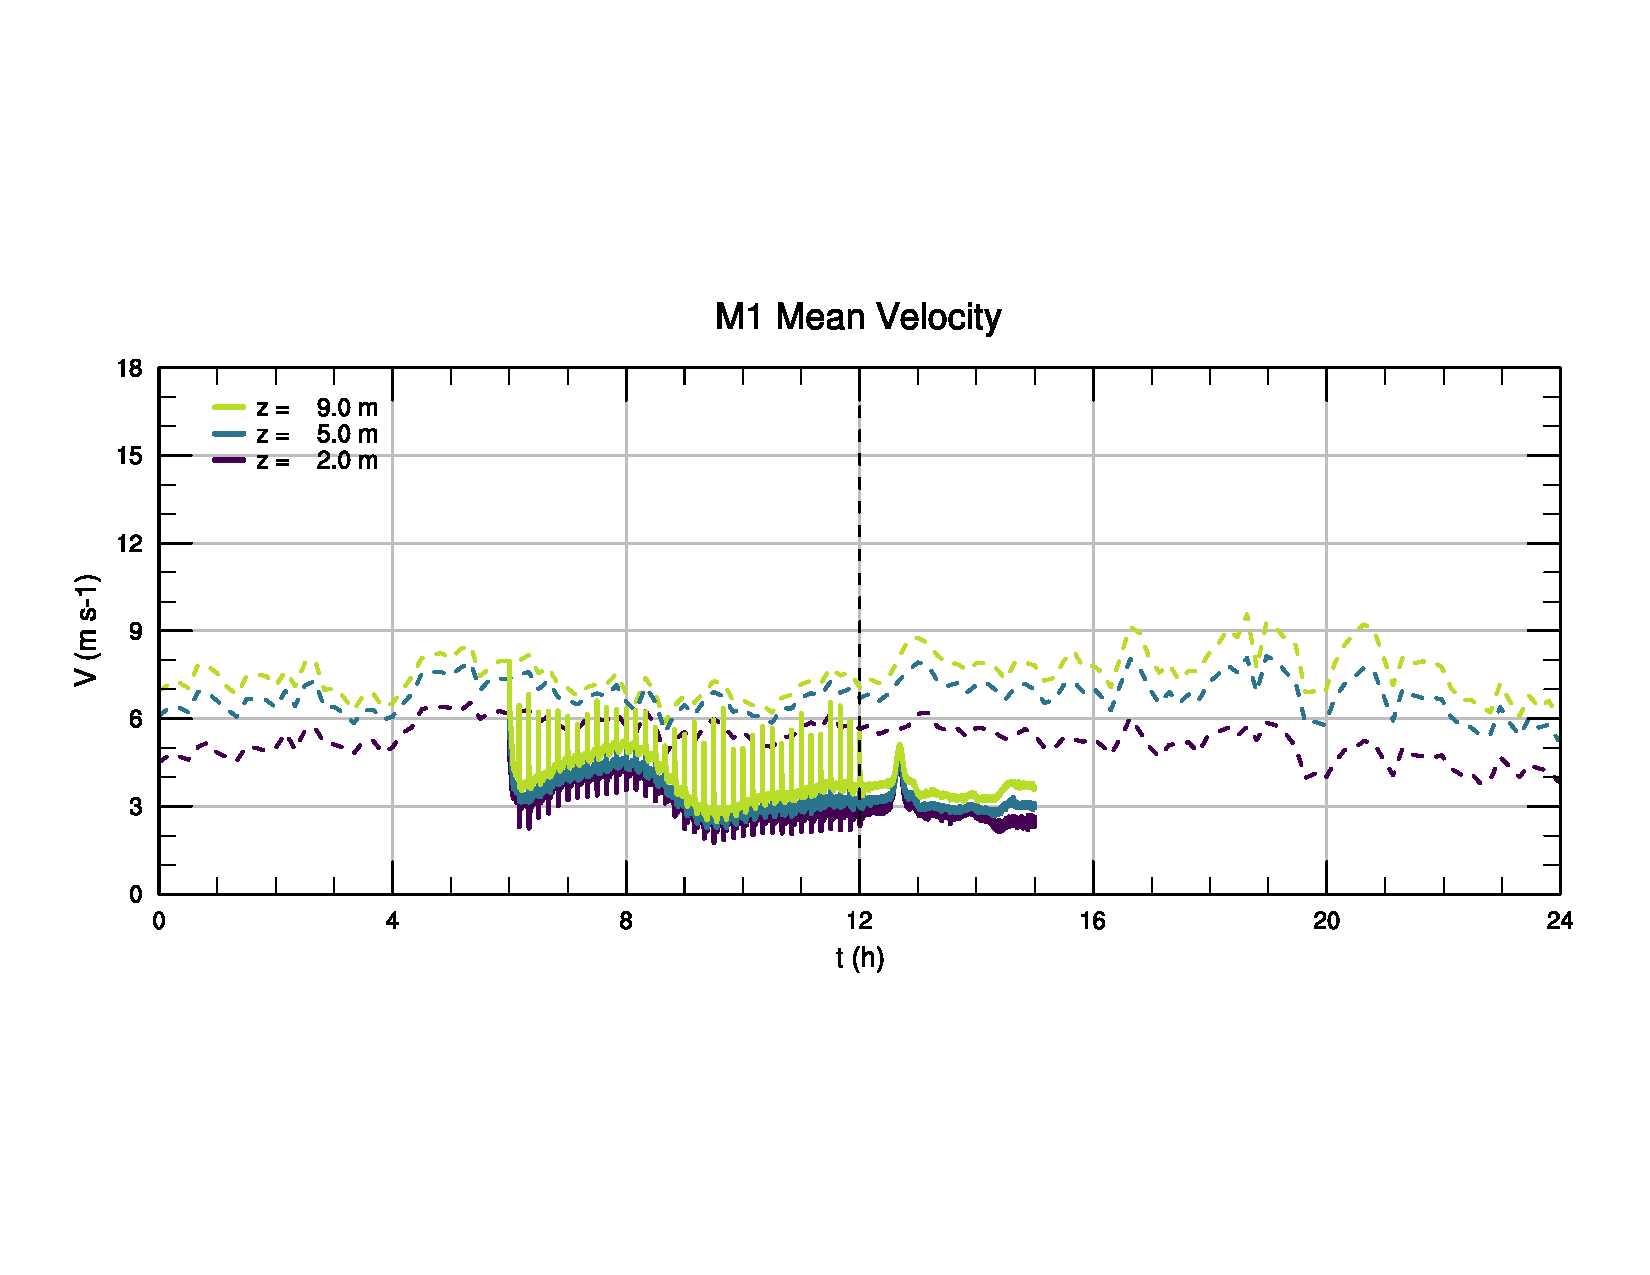
\includegraphics[width=0.87\linewidth,page=1,trim={9mm 57mm 10mm 60mm},clip]{Imagenes/06/bol/ts_interpol_compare.pdf}\\%
	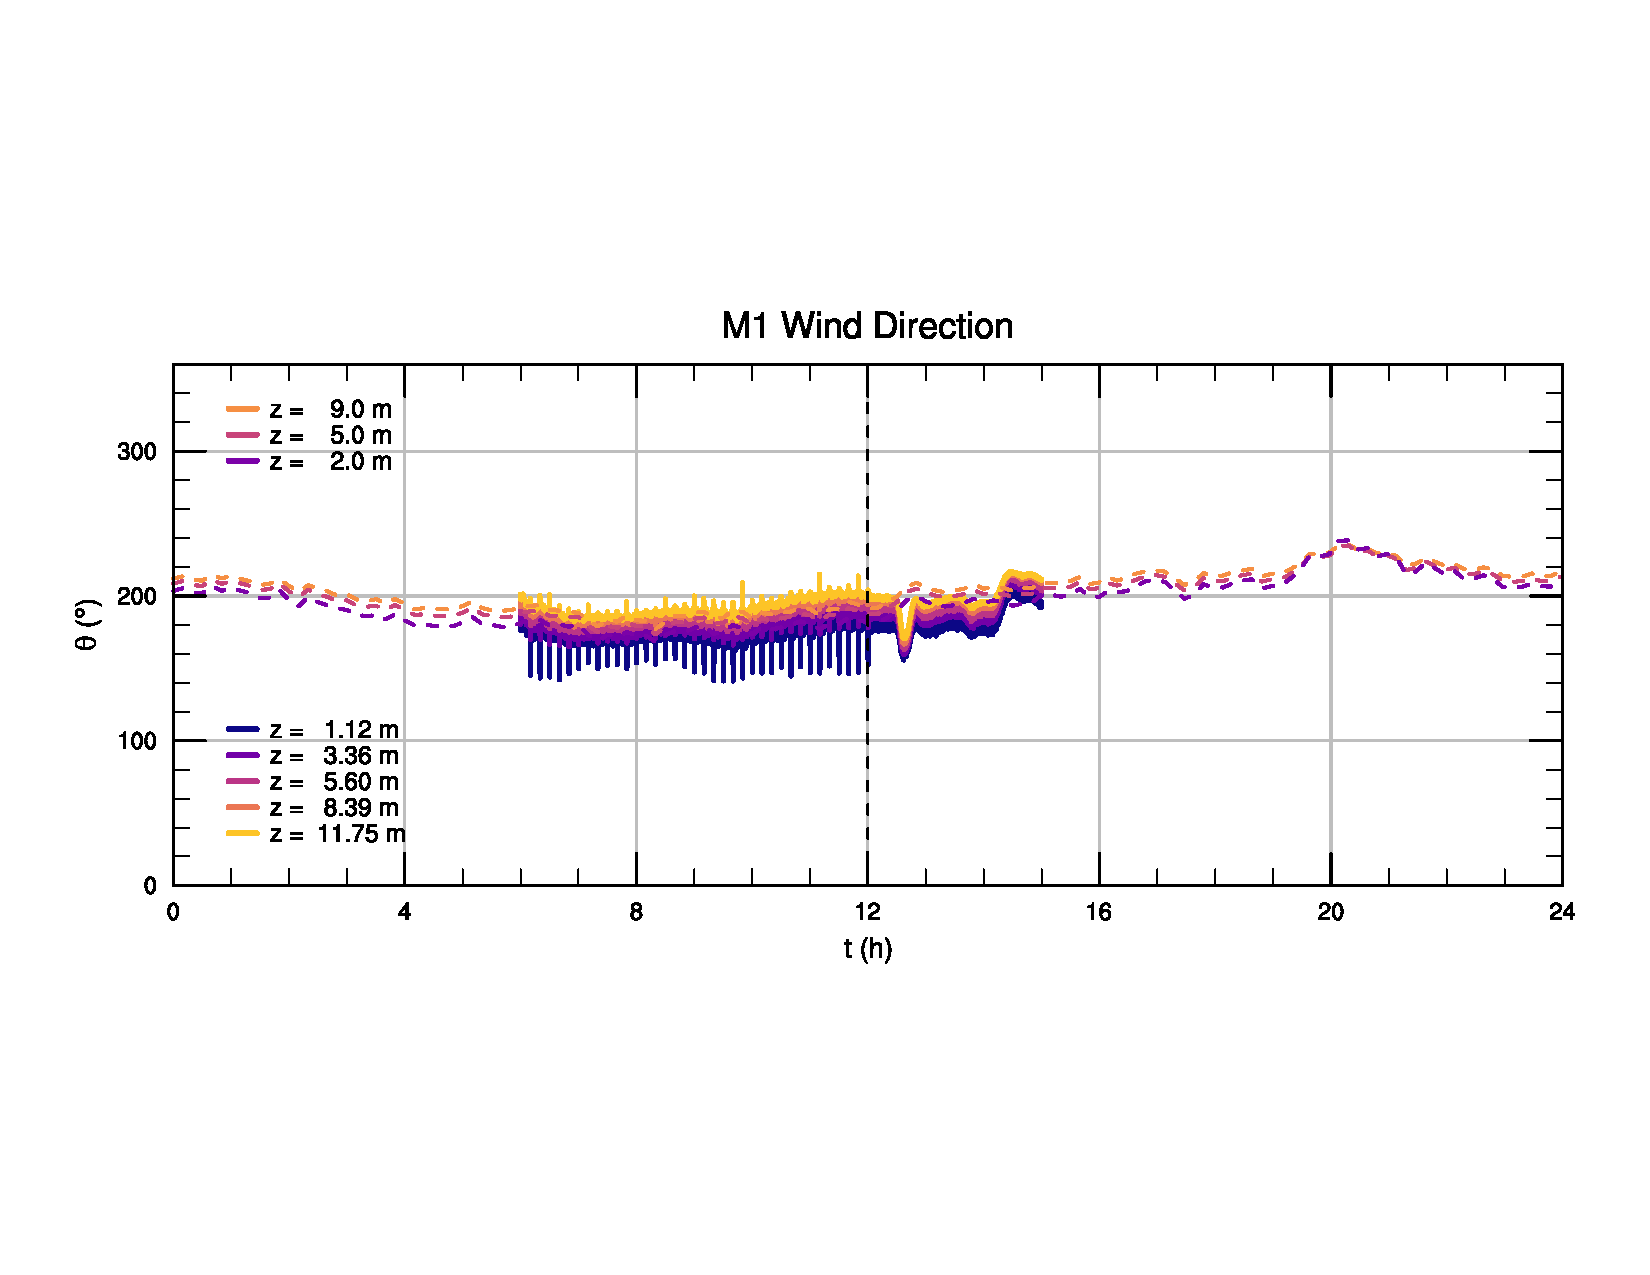
\includegraphics[width=0.87\linewidth,page=1,trim={12mm 52mm 10mm 60mm},clip]{Imagenes/06/bol/ts_interpol_compare_o.pdf}%
	\vspace{-2mm}\caption{Series de tiempo para la rapidez $V$ y dirección $\theta$ del viento en M1.}
	\label{fig:06_bol_ts_m1}
\end{figure}

\begin{figure}[H]
	\centering
	\includegraphics[width=0.87\linewidth,page=2,trim={9mm 57mm 10mm 60mm},clip]{Imagenes/06/bol/ts_interpol_compare.pdf}\\%
	\includegraphics[width=0.87\linewidth,page=2,trim={12mm 52mm 10mm 60mm},clip]{Imagenes/06/bol/ts_interpol_compare_o.pdf}%
	\vspace{-2mm}\caption{Series de tiempo para la rapidez $V$ y dirección $\theta$ del viento en M2.}
	\label{fig:06_bol_ts_m2}
\end{figure}

\begin{figure}[H]
	\centering
	\includegraphics[width=0.87\linewidth,page=3,trim={9mm 57mm 10mm 60mm},clip]{Imagenes/06/bol/ts_interpol_compare.pdf}\\%
	\includegraphics[width=0.87\linewidth,page=3,trim={12mm 52mm 10mm 60mm},clip]{Imagenes/06/bol/ts_interpol_compare_o.pdf}%
	\vspace{-2mm}\caption{Series de tiempo para la rapidez $V$ y dirección $\theta$ del viento en M3.}
	\label{fig:06_bol_ts_m3}
\end{figure}

\begin{figure}[H]
	\centering
	\includegraphics[width=0.87\linewidth,page=4,trim={9mm 57mm 10mm 60mm},clip]{Imagenes/06/bol/ts_interpol_compare.pdf}\\%
	\includegraphics[width=0.87\linewidth,page=4,trim={12mm 52mm 10mm 60mm},clip]{Imagenes/06/bol/ts_interpol_compare_o.pdf}%
	\vspace{-2mm}\caption{Series de tiempo para la rapidez $V$ y dirección $\theta$ del viento en M4.}
	\label{fig:06_bol_ts_m4}
\end{figure}

\begin{figure}[H]
	\centering
	\includegraphics[width=0.87\linewidth,page=5,trim={9mm 57mm 10mm 60mm},clip]{Imagenes/06/bol/ts_interpol_compare.pdf}\\%
	\includegraphics[width=0.87\linewidth,page=5,trim={12mm 52mm 10mm 60mm},clip]{Imagenes/06/bol/ts_interpol_compare_o.pdf}%
	\vspace{-2mm}\caption{Series de tiempo para la rapidez $V$ y dirección $\theta$ del viento en M5.}
	\label{fig:06_bol_ts_m5}
\end{figure}

\begin{figure}[H]
	\centering
	\includegraphics[width=0.87\linewidth,page=6,trim={9mm 57mm 10mm 60mm},clip]{Imagenes/06/bol/ts_interpol_compare.pdf}\\%
	\includegraphics[width=0.87\linewidth,page=6,trim={12mm 52mm 10mm 60mm},clip]{Imagenes/06/bol/ts_interpol_compare_o.pdf}%
	\vspace{-2mm}\caption{Series de tiempo para la rapidez $V$ y dirección $\theta$ del viento en M6.}
	\label{fig:06_bol_ts_m6}
\end{figure}

\begin{figure}[H]
	\centering
	\includegraphics[width=0.87\linewidth,page=7,trim={9mm 57mm 10mm 60mm},clip]{Imagenes/06/bol/ts_interpol_compare.pdf}\\%
	\includegraphics[width=0.87\linewidth,page=7,trim={12mm 52mm 10mm 60mm},clip]{Imagenes/06/bol/ts_interpol_compare_o.pdf}%
	\vspace{-2mm}\caption{Series de tiempo para la rapidez $V$ y dirección $\theta$ del viento en M7.}
	\label{fig:06_bol_ts_m7}
\end{figure}

\begin{figure}[H]
	\centering
	\includegraphics[width=0.87\linewidth,page=8,trim={9mm 57mm 10mm 60mm},clip]{Imagenes/06/bol/ts_interpol_compare.pdf}\\%
	\includegraphics[width=0.87\linewidth,page=8,trim={12mm 52mm 10mm 60mm},clip]{Imagenes/06/bol/ts_interpol_compare_o.pdf}%
	\vspace{-2mm}\caption{Series de tiempo para la rapidez $V$ y dirección $\theta$ del viento en M8.}
	\label{fig:06_bol_ts_m8}
\end{figure}

\begin{figure}[H]
	\centering
	\includegraphics[width=1.0\linewidth,page=1,trim={3mm 5mm 3mm 3mm},clip]{Imagenes/06/bol/spectra}%
	\caption{Espectros de energía para la componente horizontal del viento a distintos niveles verticales en el dominio d08 caso Bolund.}
	\label{fig:06_bol_spectrum}
\end{figure}

\begin{center}
\boxed{\textbf{MAE= 2.67240, RMSE=2.95385}}
\end{center}

































\newpage
\section{Caso II: Bolund c/DA}
\begin{figure}[H]
	\begin{minipage}{0.5\linewidth}
		\centering{\hspace{0.9cm}(a)}
	\end{minipage}%
	\begin{minipage}{0.5\linewidth}
		\centering{\hspace{0.6cm}(b)}
	\end{minipage}%
	
	\begin{minipage}{0.5\linewidth}
		\centering
		\includegraphics[width=0.9\linewidth,trim={0cm 5mm 0cm 0mm},clip]{Imagenes/06/bol_da/mean_pbl}%
	\end{minipage}%
	\begin{minipage}{0.5\linewidth}
		\centering
		\includegraphics[width=0.9\linewidth,trim={0cm 5mm 0cm 0cm},clip]{Imagenes/06/bol_da/mean_profile}%
	\end{minipage}%
	
	\caption{Ciclo horario del perfil de temperatura potencial promedio de los 8 mástiles (con DA). (a) Resultados cada 10 minutos del perfil de $\theta$. (b) Corresponde al detalle del perfil dentro de la capa límite atmosférica con resultados cada 15 minutos ($\delta\approx300$ [m]).}
	\label{fig:06_bol_da_pbl}
\end{figure}

\begin{figure}[H]
	\begin{minipage}{0.5\linewidth}
		\centering
		\hspace{1cm}(a)
	\end{minipage}%
	\begin{minipage}{0.5\linewidth}
		\centering
		\hspace{-1cm}(b)
	\end{minipage}%
	
	\begin{minipage}{0.5\linewidth}
		\centering
		\includegraphics[height=0.70\linewidth,page=73,trim={12mm 31mm 50mm 20mm},clip]{Imagenes/06/bol_da/eta1}%
	\end{minipage}%
	\begin{minipage}{0.5\linewidth}
		\centering
		\includegraphics[height=0.70\linewidth,page=85,trim={37mm 31mm 20mm 20mm},clip]{Imagenes/06/bol_da/eta1}%
	\end{minipage}%
	\vspace{1mm}
	
	\begin{minipage}{0.5\linewidth}
		\centering
		\hspace{1cm}(c)
	\end{minipage}%
	\begin{minipage}{0.5\linewidth}
		\centering
		\hspace{-1cm}(d)
	\end{minipage}%
	
	\begin{minipage}{0.5\linewidth}
		\centering
		\includegraphics[height=0.73\linewidth,page=97,trim={12mm 23mm 50mm 20mm},clip]{Imagenes/06/bol_da/eta1}%
	\end{minipage}%
	\begin{minipage}{0.5\linewidth}
		\centering
		\includegraphics[height=0.73\linewidth,page=109,trim={37mm 23mm 20mm 20mm},clip]{Imagenes/06/bol_da/eta1}%
	\end{minipage}%
	\caption{Lineas de flujo para la solución numérica en Bolund (con DA) en el primer nivel ($z_1 = 1.12$ [m]) en las horas (a) 12:00, (b) 13:00, (c) 14:00, (d) 15:00.}
	\label{fig:06_bol_da_st}
\end{figure}

\begin{figure}[H]
	\centering
	\includegraphics[width=0.90\linewidth,trim={0mm 202.0mm 111mm 106mm},clip]{Imagenes/06/bol_da/1200rot}\\%
	\includegraphics[width=0.90\linewidth,trim={0mm 202.0mm 111mm 106mm},clip]{Imagenes/06/bol_da/1300rot}\\%
	\includegraphics[width=0.90\linewidth,trim={0mm 202.0mm 111mm 106mm},clip]{Imagenes/06/bol_da/1400rot}\\%
	\includegraphics[width=0.90\linewidth,trim={0mm 180.0mm 111mm 106mm},clip]{Imagenes/06/bol_da/1500rot}%
	\caption{Contornos de rapidez del viento para la sección de corte a 240$^\circ$ en Bolund (con DA). Se muestran los resultados para las 12:00, 13:00, 14:00 y 15:00 horas.}
	\label{fig:06_bol_da_cross}
\end{figure}

\begin{figure}[H]
	\begin{minipage}{0.5\linewidth}
		\centering{\hspace{0.9cm}(a)}
	\end{minipage}%
	\begin{minipage}{0.5\linewidth}
		\centering{\hspace{0.6cm}(b)}
	\end{minipage}%
	
	\begin{minipage}{0.5\linewidth}
		\centering
		\includegraphics[width=0.7\linewidth,trim={4.5cm 12mm 4.3cm 20mm},clip]{Imagenes/06/bol_da/V_referencia}%
	\end{minipage}%
	\begin{minipage}{0.5\linewidth}
		\centering
		\includegraphics[width=0.7\linewidth,trim={4.5cm 12mm 4.3cm 20mm},clip]{Imagenes/06/bol_da/tke_referencia}%
	\end{minipage}%
	
	\caption{Perfiles promedio referenciales (Bolund con DA) en el flujo no perturbado para: (a) Rapidez del viento (en línea punteada se presenta la condición de contorno presentada por Bechmann et. al., 2011) (b) Intensidad de energía cinética turbulenta (sgs).}
	\label{fig:06_bol_da_referencia}
\end{figure}

\begin{figure}[H]
	\centering
	\includegraphics[width=0.95\linewidth,trim={12mm 84mm 10mm 74mm},page=1,clip]{Imagenes/06/bol_da/speedup}\\%
	\includegraphics[width=0.95\linewidth,trim={12mm 84mm 10mm 74mm},page=13,clip]{Imagenes/06/bol_da/speedup}\\%
	\includegraphics[width=0.95\linewidth,trim={12mm 84mm 10mm 74mm},page=25,clip]{Imagenes/06/bol_da/speedup}\\%
	\includegraphics[width=0.95\linewidth,trim={12mm 84mm 10mm 74mm},page=37,clip]{Imagenes/06/bol_da/speedup}\\%
	\includegraphics[width=0.95\linewidth,trim={-11mm 193mm 115mm 112mm},clip]{Imagenes/06/bol_da/cross_height}\\%
	\caption{Speedup en los primeros 3 niveles del modelo ($1.1$ [m] azul; $3.4$ [m] verde; $5.6$ [m] amarillo) para la sección de corte a 240$^\circ$ en Bolund (con DA). Se muestran los resultados para las 12:00, 13:00, 14:00 y 15:00 horas.}
	\label{fig:06_bol_da_speedup}
\end{figure}

\begin{figure}[H]
	\centering
	\includegraphics[width=0.90\linewidth,trim={12mm 84mm 10mm 74mm},page=1,clip]{Imagenes/06/bol_da/delta_tke}\\%
	\includegraphics[width=0.90\linewidth,trim={12mm 84mm 10mm 74mm},page=13,clip]{Imagenes/06/bol_da/delta_tke}\\%
	\includegraphics[width=0.90\linewidth,trim={12mm 84mm 10mm 74mm},page=25,clip]{Imagenes/06/bol_da/delta_tke}\\%
	\includegraphics[width=0.90\linewidth,trim={12mm 84mm 10mm 74mm},page=37,clip]{Imagenes/06/bol_da/delta_tke}\\%
	\includegraphics[width=0.90\linewidth,trim={-13.3mm 193mm 115mm 112mm},clip]{Imagenes/06/bol_da/cross_height}\\%
	\caption{Incremento adimnsional de energía cinética turbulenta (sgs) en los primeros 3 niveles del modelo ($1.1$ [m] azul; $3.4$ [m] verde; $5.6$ [m] amarillo) para la sección de corte a 240$^\circ$ en Bolund (con DA). Se muestran los resultados para las 12:00, 13:00, 14:00 y 15:00 horas.}
	\label{fig:06_bol_da_tke}
\end{figure}

\begin{figure}[H]
	\begin{minipage}{0.5\linewidth}
		\centering
		\hspace{7mm}(a)\end{minipage}%
	\begin{minipage}{0.5\linewidth}
		\centering
		\hspace{-5mm}(b)\end{minipage}%
	
	\centering
	\includegraphics[height=0.75\linewidth,page=1,trim={28mm 10mm 25mm 23mm},clip]{Imagenes/06/bol_da/V_masts}%
	\includegraphics[height=0.75\linewidth,page=1,trim={30mm 10mm 17mm 20mm},clip]{Imagenes/06/bol_da/k_masts}%
	\vspace{-2mm}\caption{Perfil vertical de (a) \emph{speedup} y (b) variación adimensional de energía cinética turbulenta para M1 (púrpura), M2 (azul), M3 (turquesa) y M4 (verde) para el caso con DA.}
	\label{fig:06_bol_da_mast_tke_speedup}
\end{figure}

\begin{figure}[H]
	\centering
	\includegraphics[width=0.87\linewidth,page=1,trim={9mm 57mm 10mm 60mm},clip]{Imagenes/06/bol_da/ts_interpol_compare.pdf}\\%
	\includegraphics[width=0.87\linewidth,page=1,trim={12mm 52mm 10mm 60mm},clip]{Imagenes/06/bol_da/ts_interpol_compare_o.pdf}%
	\vspace{-2mm}\caption{Series de tiempo para la rapidez $V$ y dirección $\theta$ del viento en M1 con DA.}
	\label{fig:06_bol_da_ts_m1}
\end{figure}

\begin{figure}[H]
	\centering
	\includegraphics[width=0.87\linewidth,page=2,trim={9mm 57mm 10mm 60mm},clip]{Imagenes/06/bol_da/ts_interpol_compare.pdf}\\%
	\includegraphics[width=0.87\linewidth,page=2,trim={12mm 52mm 10mm 60mm},clip]{Imagenes/06/bol_da/ts_interpol_compare_o.pdf}%
	\vspace{-2mm}\caption{Series de tiempo para la rapidez $V$ y dirección $\theta$ del viento en M2 con DA.}
	\label{fig:06_bol_da_ts_m2}
\end{figure}

\begin{figure}[H]
	\centering
	\includegraphics[width=0.87\linewidth,page=3,trim={9mm 57mm 10mm 60mm},clip]{Imagenes/06/bol_da/ts_interpol_compare.pdf}\\%
	\includegraphics[width=0.87\linewidth,page=3,trim={12mm 52mm 10mm 60mm},clip]{Imagenes/06/bol_da/ts_interpol_compare_o.pdf}%
	\vspace{-2mm}\caption{Series de tiempo para la rapidez $V$ y dirección $\theta$ del viento en M3 con DA.}
	\label{fig:06_bol_da_ts_m3}
\end{figure}

\begin{figure}[H]
	\centering
	\includegraphics[width=0.87\linewidth,page=4,trim={9mm 57mm 10mm 60mm},clip]{Imagenes/06/bol_da/ts_interpol_compare.pdf}\\%
	\includegraphics[width=0.87\linewidth,page=4,trim={12mm 52mm 10mm 60mm},clip]{Imagenes/06/bol_da/ts_interpol_compare_o.pdf}%
	\vspace{-2mm}\caption{Series de tiempo para la rapidez $V$ y dirección $\theta$ del viento en M4 con DA.}
	\label{fig:06_bol_da_ts_m4}
\end{figure}

\begin{figure}[H]
	\centering
	\includegraphics[width=0.87\linewidth,page=5,trim={9mm 57mm 10mm 60mm},clip]{Imagenes/06/bol_da/ts_interpol_compare.pdf}\\%
	\includegraphics[width=0.87\linewidth,page=5,trim={12mm 52mm 10mm 60mm},clip]{Imagenes/06/bol_da/ts_interpol_compare_o.pdf}%
	\vspace{-2mm}\caption{Series de tiempo para la rapidez $V$ y dirección $\theta$ del viento en M5 con DA.}
	\label{fig:06_bol_da_ts_m5}
\end{figure}

\begin{figure}[H]
	\centering
	\includegraphics[width=0.87\linewidth,page=6,trim={9mm 57mm 10mm 60mm},clip]{Imagenes/06/bol_da/ts_interpol_compare.pdf}\\%
	\includegraphics[width=0.87\linewidth,page=6,trim={12mm 52mm 10mm 60mm},clip]{Imagenes/06/bol_da/ts_interpol_compare_o.pdf}%
	\vspace{-2mm}\caption{Series de tiempo para la rapidez $V$ y dirección $\theta$ del viento en M6 con DA.}
	\label{fig:06_bol_da_ts_m6}
\end{figure}

\begin{figure}[H]
	\centering
	\includegraphics[width=0.87\linewidth,page=7,trim={9mm 57mm 10mm 60mm},clip]{Imagenes/06/bol_da/ts_interpol_compare.pdf}\\%
	\includegraphics[width=0.87\linewidth,page=7,trim={12mm 52mm 10mm 60mm},clip]{Imagenes/06/bol_da/ts_interpol_compare_o.pdf}%
	\vspace{-2mm}\caption{Series de tiempo para la rapidez $V$ y dirección $\theta$ del viento en M7 con DA.}
	\label{fig:06_bol_da_ts_m7}
\end{figure}

\begin{figure}[H]
	\centering
	\includegraphics[width=0.87\linewidth,page=8,trim={9mm 57mm 10mm 60mm},clip]{Imagenes/06/bol_da/ts_interpol_compare.pdf}\\%
	\includegraphics[width=0.87\linewidth,page=8,trim={12mm 52mm 10mm 60mm},clip]{Imagenes/06/bol_da/ts_interpol_compare_o.pdf}%
	\vspace{-2mm}\caption{Series de tiempo para la rapidez $V$ y dirección $\theta$ del viento en M8 con DA.}
	\label{fig:06_bol_da_ts_m8}
\end{figure}

\begin{figure}[H]
	\centering
	\includegraphics[width=1.0\linewidth,page=1,trim={3mm 5mm 3mm 3mm},clip]{Imagenes/06/bol_da/spectra}%
	\caption{Espectros de energía para la componente horizontal del viento a distintos niveles verticales en el dominio d08 caso Bolund con DA.}
	\label{fig:06_bol_da_spectrum}
\end{figure}

\begin{center}
	\boxed{\textbf{MAE= --, RMSE= --}}
\end{center}
